\section{SeismicDarts}\label{sec:SeismicDarts}

A SeismicDart combines a geophone (GS-100) with the fins and body of a lawn Jart\textsuperscript{TM}, using a 3D-printed chamber that encloses a WiFi-enabled microcontroller (particle.io Photon\textsuperscript{TM}) as shown in Fig.~\ref{fig:Smart_Dart_overview}. 
The center of the chamber is slotted to fit a wooden plate holding an accelerometer that transmits data wirelessly through the microcontroller. 
The centered accelerometer card allows placing the microcontroller and battery on opposite sides, balancing the dart.
Designs and instructions to build a SeismicDart are available at \cite{Victor2016Thingiverse}.



\begin{figure} \centering
{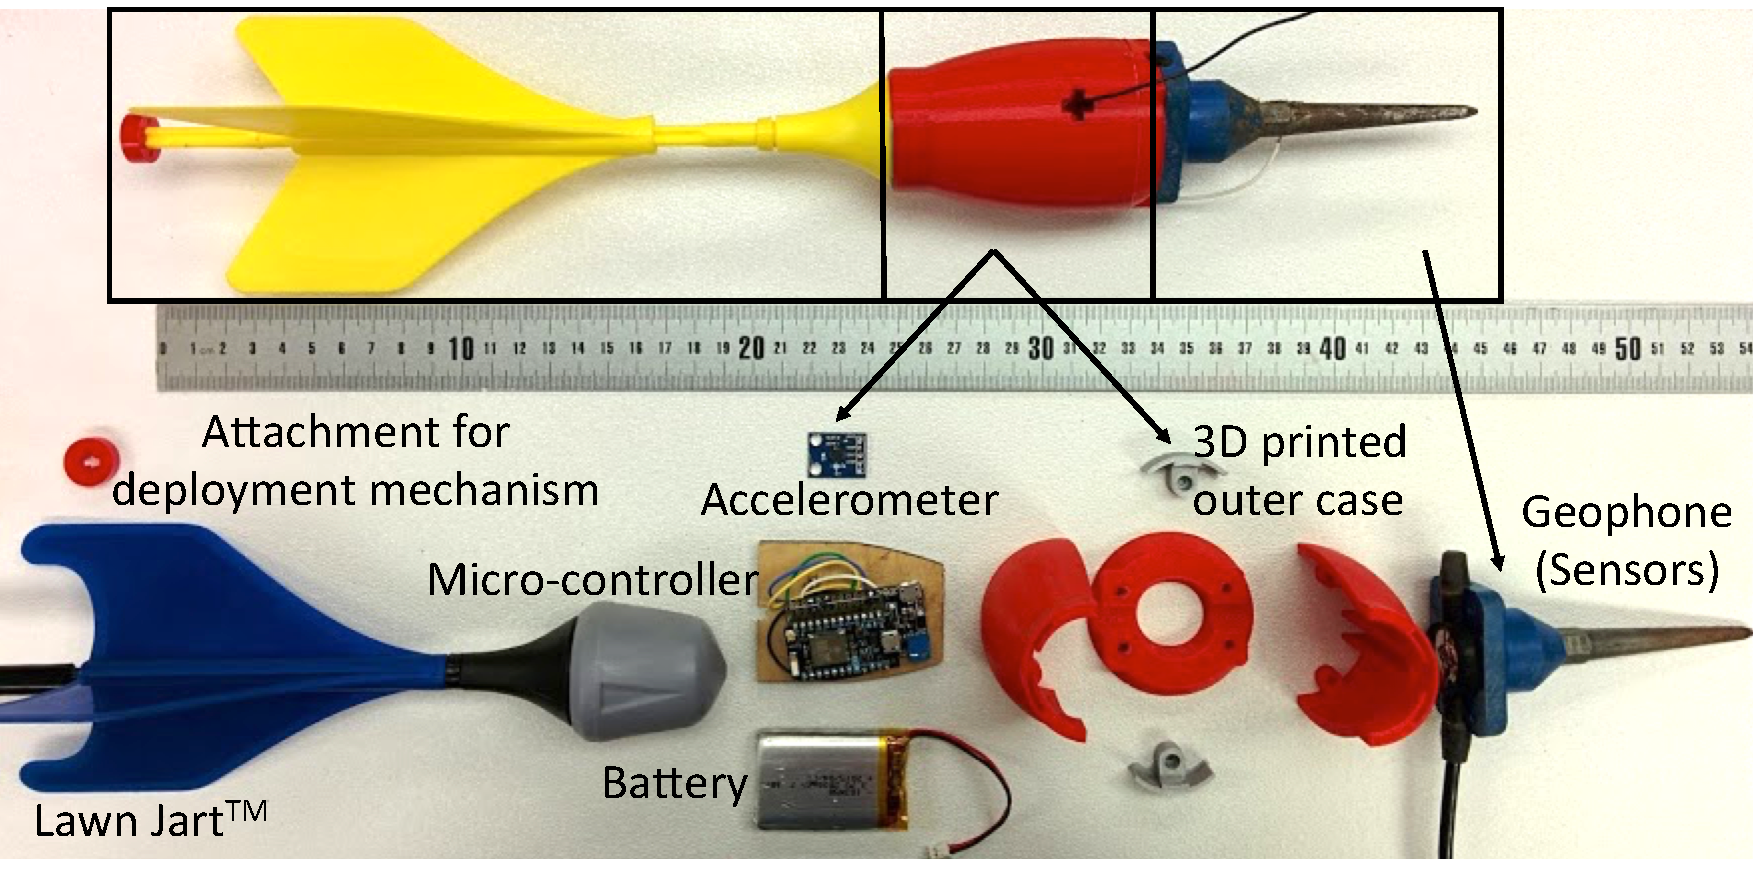
\includegraphics[width=\columnwidth]{Smart_Dart_overview.pdf}}
\caption{Components of the SeismicDart sensor: a lawn  Jart\textsuperscript{TM} fin, particle.io Photon\textsuperscript{TM}  micro-controller, 3D printed protective casing, and a geophone.} 
\label{fig:Smart_Dart_overview}
\end{figure}

%%%%%%%%%%%%%%%%%%%%%%%%%%%%%%%%%%%%%%% 
\subsection{Experiments} 
The following sections compare SeismicDart performance.
\subsubsection{ Drop tests in different soils}  


Proper planting of a geophone requires good contact with the soil and the geophone to be in a vertical position. 
Geophone protocol classifies a geophone as well planted if the angle of deviation is less than 10$^\circ$ and the spike has at least 40 mm of penetration.

To determine how SeismicDarts perform in different soils, this experiment measured penetration depth and angle of deviation in seven different soil types as a function of drop height. 
 The soil types were categorized by their compression strength, in kg/cm$^2$, measured using a soil pocket penetrometer (CertifiedMTP). Measurements for compression strength vary with small deviation in measurement location, so we repeated this measurement 10 times at 10 different locations in each soil type and computed the average.
 
 Experiments were conducted using the Seismic UAV to autonomously drop a payload of four SeismicDarts at a desired drop height. 
 Tests were conducted at drop heights of 10, 15, 20, and 25 m. 
 We measured angle of deviation and penetration depth for each drop.
 The angular deviation was recorded using two protractors.
 To measure penetration depth, the buried darts were marked where the spike met the soil, the dart was then pulled from the soil, and the distance from the spike tip to the marking was measured with calipers. 
  We repeated this measurement 12 times for each soil type at each drop height.  The soil compression strengths in these experiments ranged from 0.056 kg/cm$^2$ for river sand, to 4 kg/cm$^2$ for a hard-packed soccer field.

The four soil types with the lowest soil compression strength could be well-planted with low drop heights, so these tests were performed manually.
   Testing was performed by holding a dart at the tip opposite to the spike in a vertical position and releasing it at varying heights into 19 liter (5 gal.) buckets of soil. 

%Penetration depth and angular deviation were measured. %To measure penetration depth, the buried darts were marked where the spike met the soil, the dart was then pulled from the soil, and the distance from the spike tip to the marking was measured with calipers. The angular deviation was recorded using the accelerometer inside the dart.

 
  % These experiments shows that increasing drop height increases penetration on all soils tested.
  % Also, darts dropped in quiescent air remain vertical if they penetrate the soil.
Experiment results plotting penetration depth as a function of drop height are displayed in Fig.~\ref{fig:DepthPlotIndoors}, and angle of deviation as a function of drop height in Fig.~\ref{fig:AnglePlotIndoors}.   Both graphs are annotated with values for soil compression strength. 

\begin{figure} \centering
{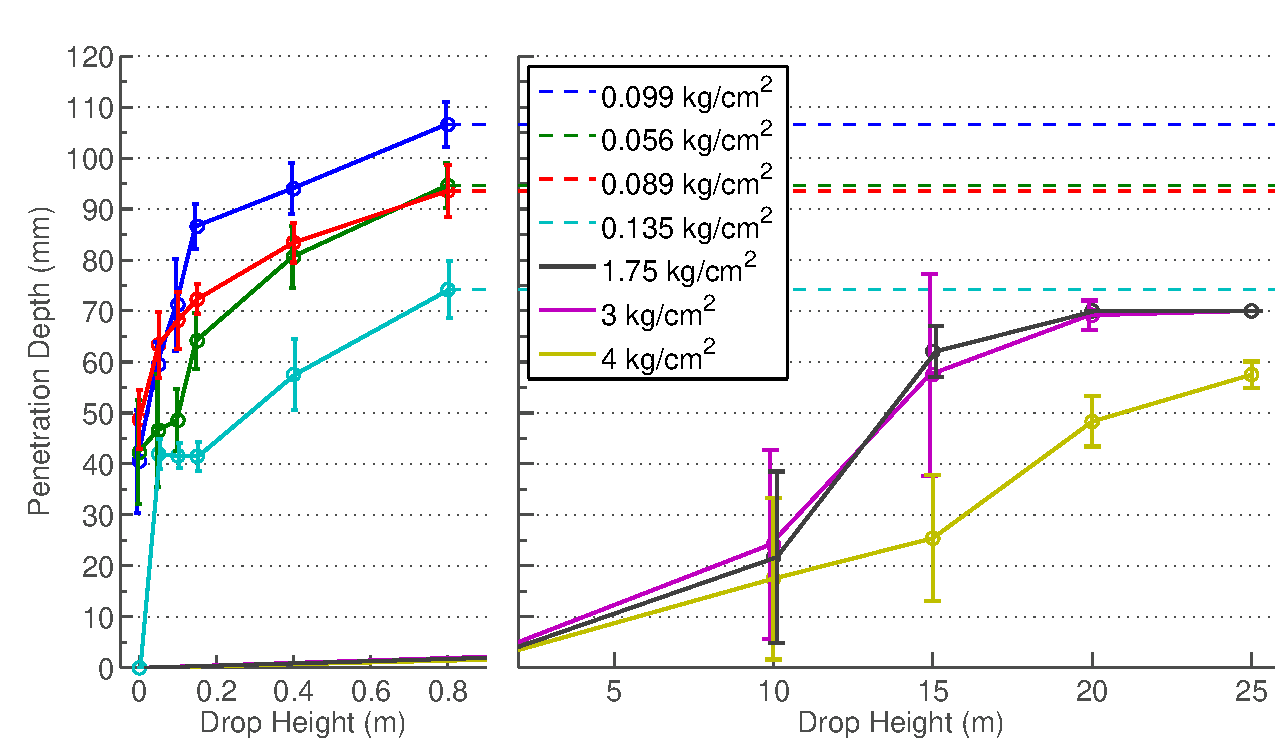
\includegraphics[width=\columnwidth]{AutoPenetrationDepth.pdf}}
\caption{Drop height vs. penetration depth in seven soil types. Drops were performed autonomously and each data point represents 12 trials. Increasing the drop height increased the penetration depth for all seven soil types.} 
\label{fig:DepthPlotIndoors}
\end{figure}

\begin{figure} \centering
{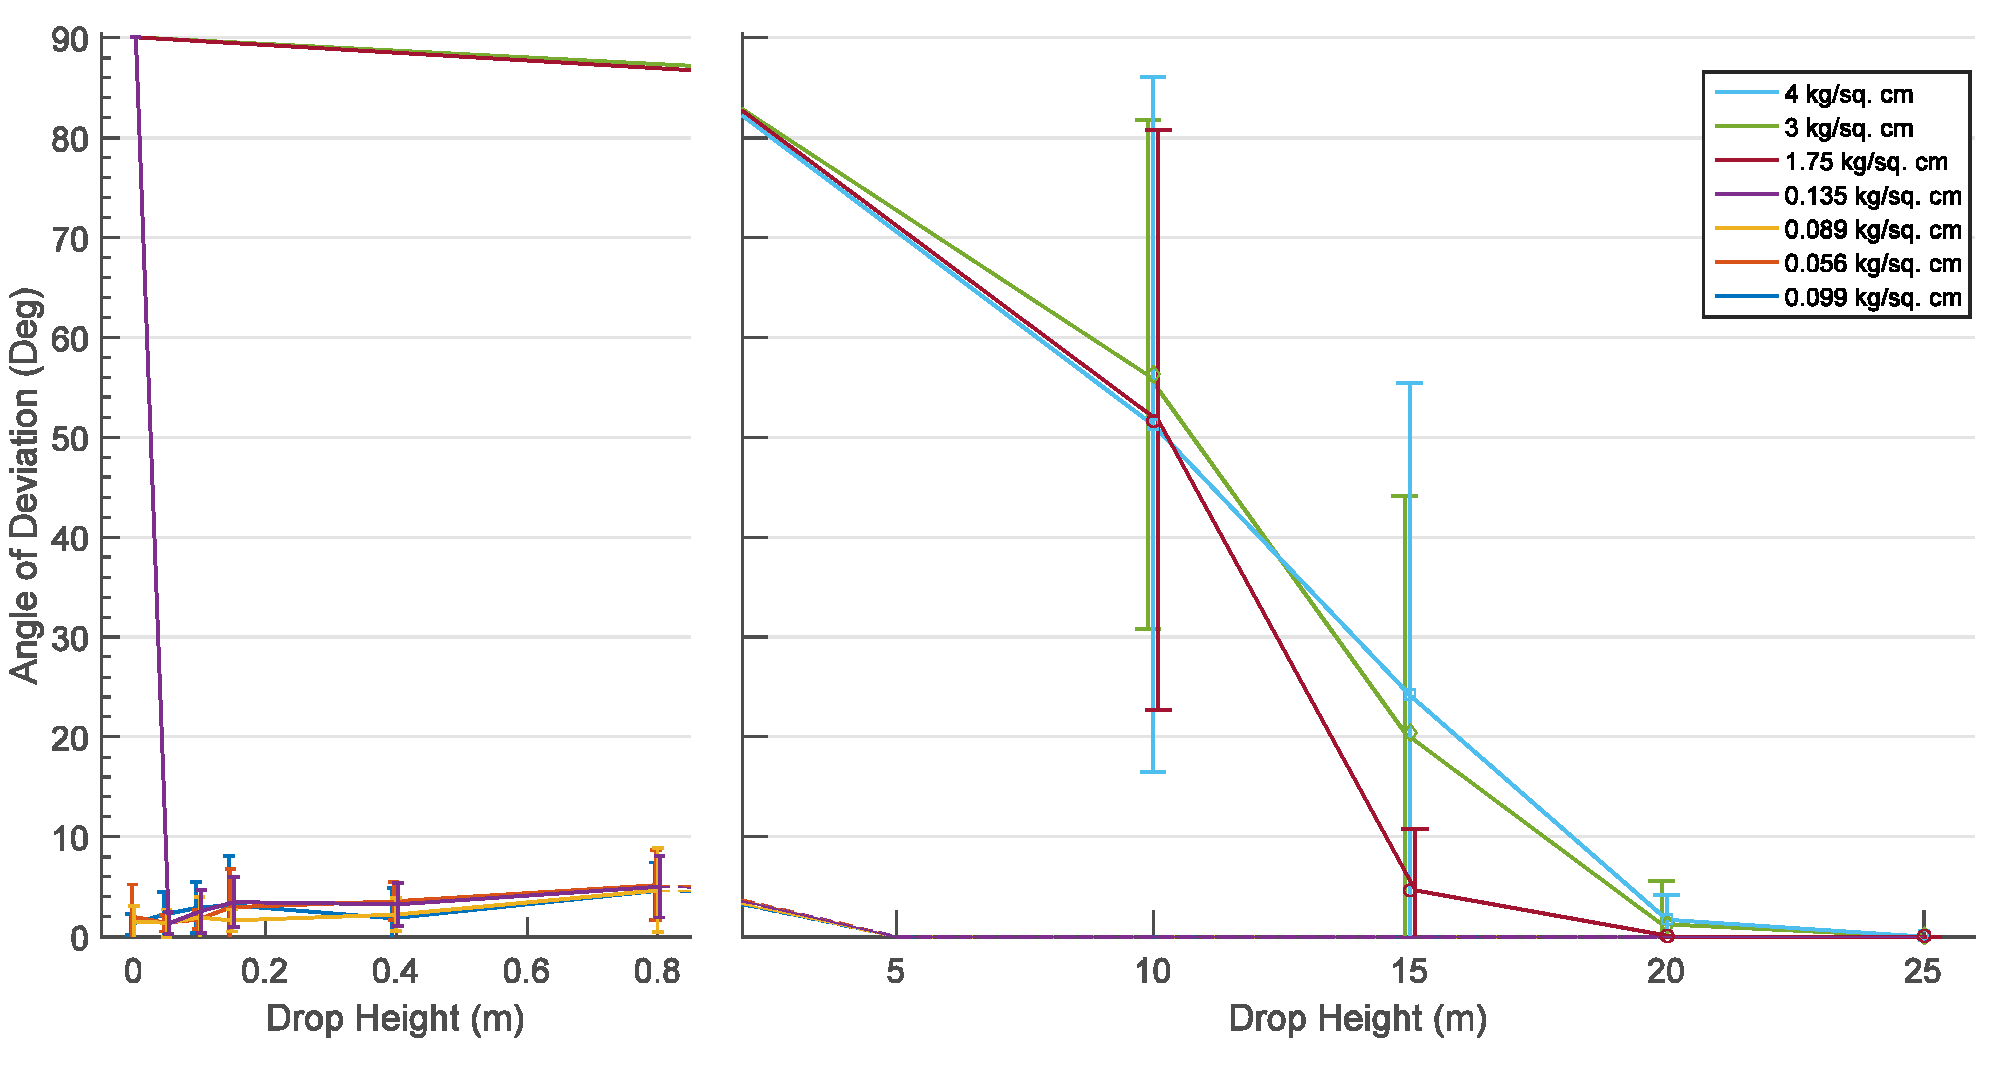
\includegraphics[width=\columnwidth]{AutoPenetrationAngle.pdf}}
\caption{Drop height vs. angle of deviation in seven soil types. Drops were performed autonomously and each data point represents 12 trials. Increasing the drop height reduced the angle of deviation for all seven soil types.} 
\label{fig:AnglePlotIndoors}
\vspace{-1em}
\end{figure}

If a SeismicDart is dropped from a sufficient height into penetrable soil, the spike will be buried into the soil, and the geophone will have small angular deviation from vertical. Soils with higher compression strength require higher drop heights. Error bars show that variance decreases with drop height for both angle of deviation and penetration depth.  
 All drops from heights 20 m or more achieved the goals of an angle of deviation less than 10$^\circ$ and a penetration at least 40 mm of penetration.   

The autonomous tests were conducted with 16 km/hr winds, demonstrating that drop heights 20 m or higher were sufficient to counter disturbances from wind. %https://www.windfinder.com/forecast/galveston_airport





%\subsubsection{Straight vs.\ Twisted Fins}

%To determine the difference in performance between SeismicDarts with straight fins and twisted fins, we ran a drop test with 10 trials for both types of dart at a constant height in one soil type. Each trial was initialized by holding the dart horizontally at a height of 9.8 meters, dropping it into the soil, and recording the penetration depth and angular deviation. Holding the darts horizontally emphasized the angle-correcting behavior of the fins. The penetration depth and angular penetration were measured and recorded as in the previous experiment. A graph showing the values recorded for penetration depth and angular deviation in Fig.~\ref{fig:StraightBentDepth}  reveals that SeismicDarts with twisted fins had less angular deviation, but also less penetration depth. 

%\begin{figure} \centering
 % {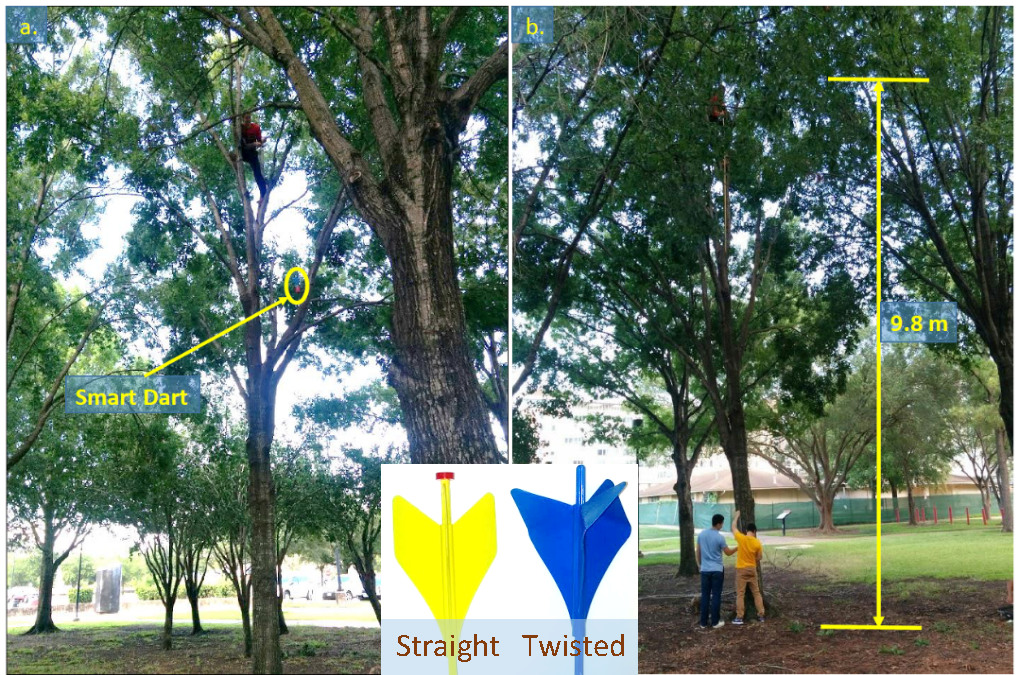
\includegraphics[width=\columnwidth]{StraightvsBent_pic.pdf}}
 %\caption{Outdoor drop test comparing straight vs.\ twisted fins performance:
 %a.)  dropping a SeismicDart,  
% b.)  measuring drop height.} 
% \label{fig:StraightBentPic}
 %\vspace{-1em}
%\end{figure}
%\begin{figure} \centering
%  {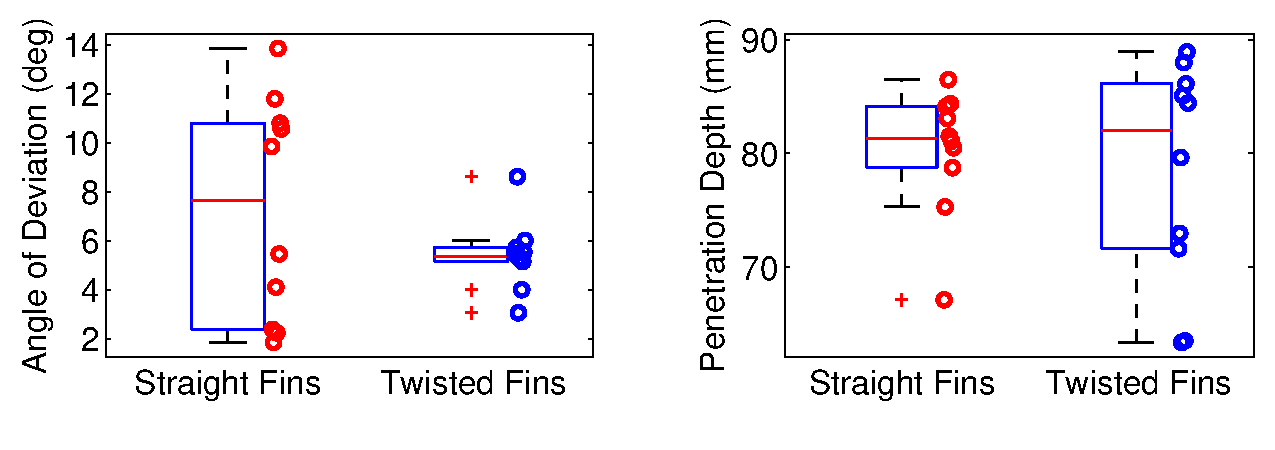
\includegraphics[width=\columnwidth]{StraightvsTwistedAngleDepth.pdf}}
% \caption{\label{fig:StraightBentDepth}Straight vs.\ twisted fins comparing a.) penetration depth b.) angle of deviation. Experiment used a fixed drop height of 9.8 m.} 
%\end{figure}

%\begin{figure}\centering 
%\subfigure[\label{subfig:StraightBentDepth}]
%  {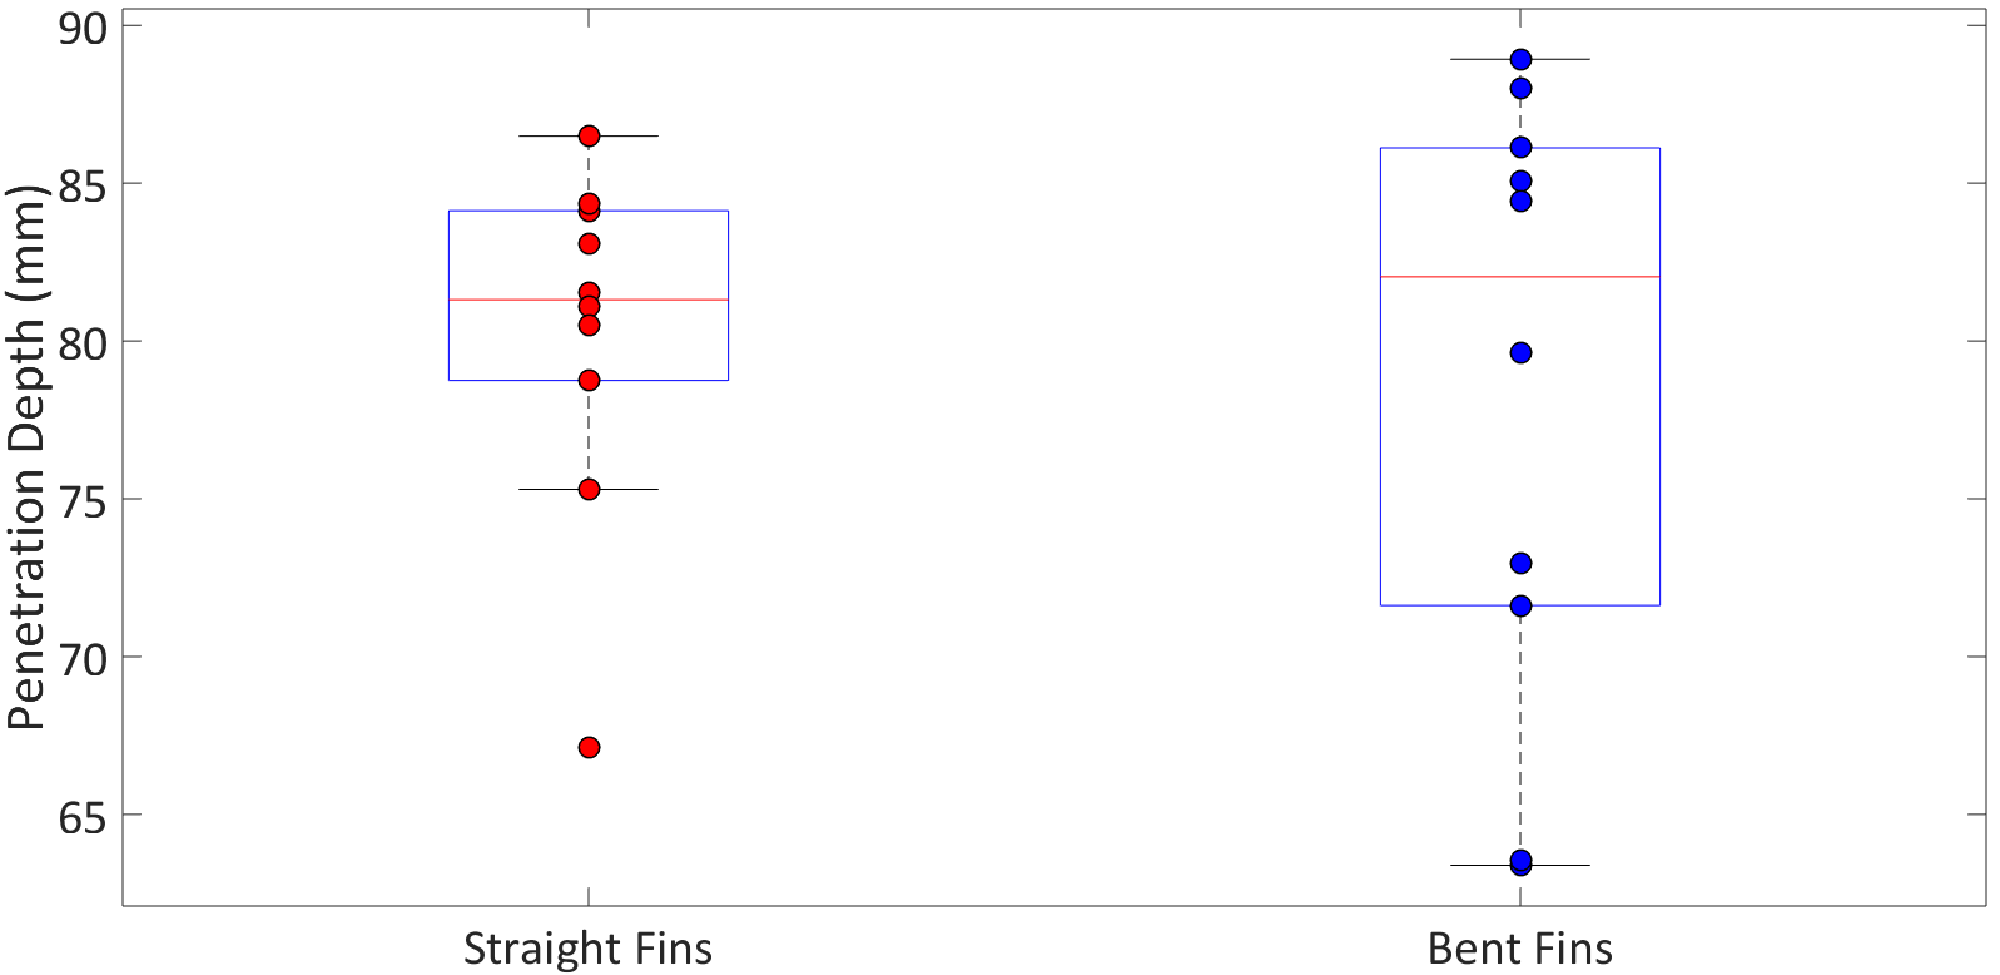
\includegraphics[width=.45\columnwidth]{StraightvsBent_depth.pdf}}
% \subfigure[\label{subfig:StraightBentAngle}]
%  {\includegraphics[width=.45\columnwidth]%{StraightvsBent_angle.pdf}}
%   \vspace*{-.1in}
 %\caption{Straight vs Bent fins comparing a.) Penetration Depth b.) Angle of Deviation. Experiment used a fixed drop height of 9.8 m. \label{fig:StraightBent}}
 %\vspace*{-.1in} 
%\end{figure} 
\subsubsection{Shot gather comparison} 
Seismic explorations use thousands of geophones to conduct a seismic survey. 
 As a proof-of-concept, this experiment ran a small-scale seismic survey to compare the performance of a traditional cabled four geophone system with readings from four autonomously deployed SeismicDarts.
Flying autonomously at a drop height of 25 m, the Seismic UAV flew to GPS waypoints spaced 4 m apart and deployed one dart at each location. 
A seismic survey technician manually planted four traditional cabled geophones, each 10 cm from a deployed SeismicDart. 
A seismic wave was generated using a sledge hammer hitting a steel plate.

Results of the field test comparison between the traditional cabled geophone system and the SeismicDarts are shown in Fig.~\ref{fig:shotgather_auto_drop}.   
Data were obtained using a \emph{Strata-Visor}, a device that can obtain, store, and plot the sensed data. 
The \emph{Strata-Visor} is extensively used with traditional geophone setups because the geophones can only sense vibrational waves and are dependent on other devices for storage and data processing. 
To allow a fair comparison, the SeismicDart's  ability to store sensed data was not used in this experiment. 
 The \emph{Strata-Visor} records the geophone voltage at 2000 Hz, using an 24 bit ADC.

The readings from both systems are qualitatively similar, with no discernible phase or amplitude differences. Let $X$ be measurements from the traditional geophone and $Y$ the corresponding voltages from a SmartDart.
The percent peak-to-peak error and normalized root-mean-square error (NRMSE) are defined as
\begin{align}
e_{pp} &= 100 \left( \frac{ \max(X) - \min(X) }{ \max(Y) - \min(Y) } -1\right) \\
  \text{NRMSE} &=\frac{100}{\max(X) - \min(X)} \sqrt{ \frac{ \sum_{i=1}^n \left( X(i) - Y(i) \right)}{n} }.\nonumber
\end{align}
The peak-to-peak errors were [-6.33, -1.15, -1.81,  9.84] \% for sensors at [4,8,12,16] m from the source.
 The NRMSE were [1.05,1.27,3.98,4.39] \% for sensors at [4,8,12,16] m from the source.
%$e_{\text{4 m}}  =  -6.3 \%, e_{\text{8 m}}  =  11.93 \%, e_{\text{12 m}}  = -1.81\%, e_{\text{16 m}}  = 0.981 \%$. 
%The RMSD error were $RMSD_{\text{4 m}}  =  -6.3 \%, RMSD_{\text{8 m}}  =  11.93 \%, RMSD_{\text{12 m}}  = \%, RMSD_{\text{16 m}}  = 0.981 \%$. 
Readings were also compared using a Pearson product-moment correlation coefficient, which gives a correlation measurement between $-1$ and $+1$ where $+1$ is total positive linear correlation.
\begin{align}
\rho_{X,Y} = \frac{E\left[  (X-\mu_X) (Y-\mu_Y)  \right]}{  \sigma_X, \sigma_Y}
\end{align}

The correlation coefficients were $\rho_{\text{4 m}}  =  0.9813, \rho_{\text{8 m}}  =  0.9836, \rho_{\text{12 m}}  =  0.8600, \rho_{\text{16 m}}  = 0.8114$. These correlations decrease with distance. The SeismicDart is subject to low-amplitude noise, which is easiest to see in the fourth sensor because it was 16 m from the seismic source and thus had the lowest signal amplitude.  This noise is potentially due to wind striking the SeismicDart's fin. The effect of noise can be mitigated by using larger seismic sources such as a vibration truck or explosives.



\begin{figure} \centering
  {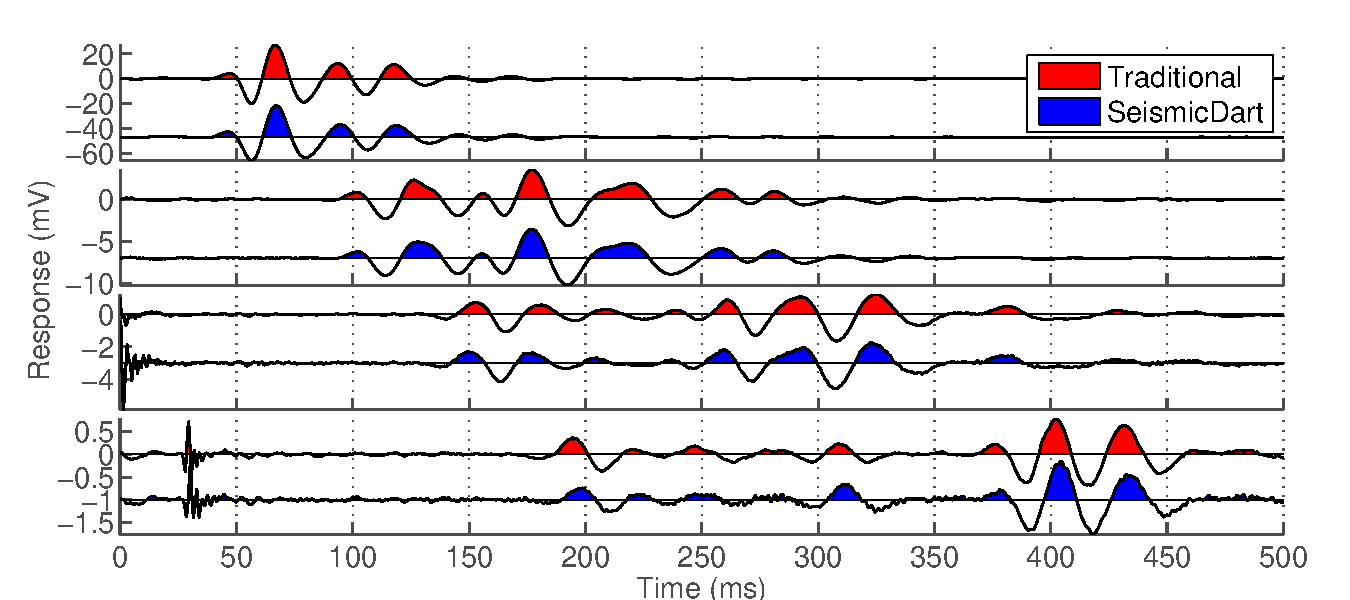
\includegraphics[width=\columnwidth]{SeismicSurveyComparison.pdf}}
 \caption{Raw voltage data from shot gather comparison of four traditional geophones and four autonomously dropped SeismicDart sensors.  
 \label{fig:shotgather_auto_drop}}
\end{figure}

\subsection{SeismicDart Deployment and Retrieval}
First the SeismicDarts are loaded onto to a UAV. 
Currently a maximum of four sensors can be dropped in a single flight. 
The flight plan communicated to the UAV provides a GPS waypoint for each SmartDart. 
The UAV flies to and drops a SmartDart at each waypoint, then returns home. 

Deployment is only one part of a survey. Large surveys require moving and reusing sensors.  
Because SmartDarts are more expensive than standard geophones, rapid reuse is essential.
The UAV has an underslung hook for picking up a SeismicDart.
Retrieval is facilitated by attaching a wire loop to the SeismicDart tail, which provide a target 300 mm in diameter for the hook.
Currently retrieval is performed by manually piloting the UAV, but this level of accuracy is within the accuracy of UAVS equipped with RTK GPS.
Automating retrieval is out of the scope of this paper.
Fig.~\ref{fig:SeismicDart_DR} shows a SeismicDart being retrieved and redeployed.


\begin{figure} \centering
  {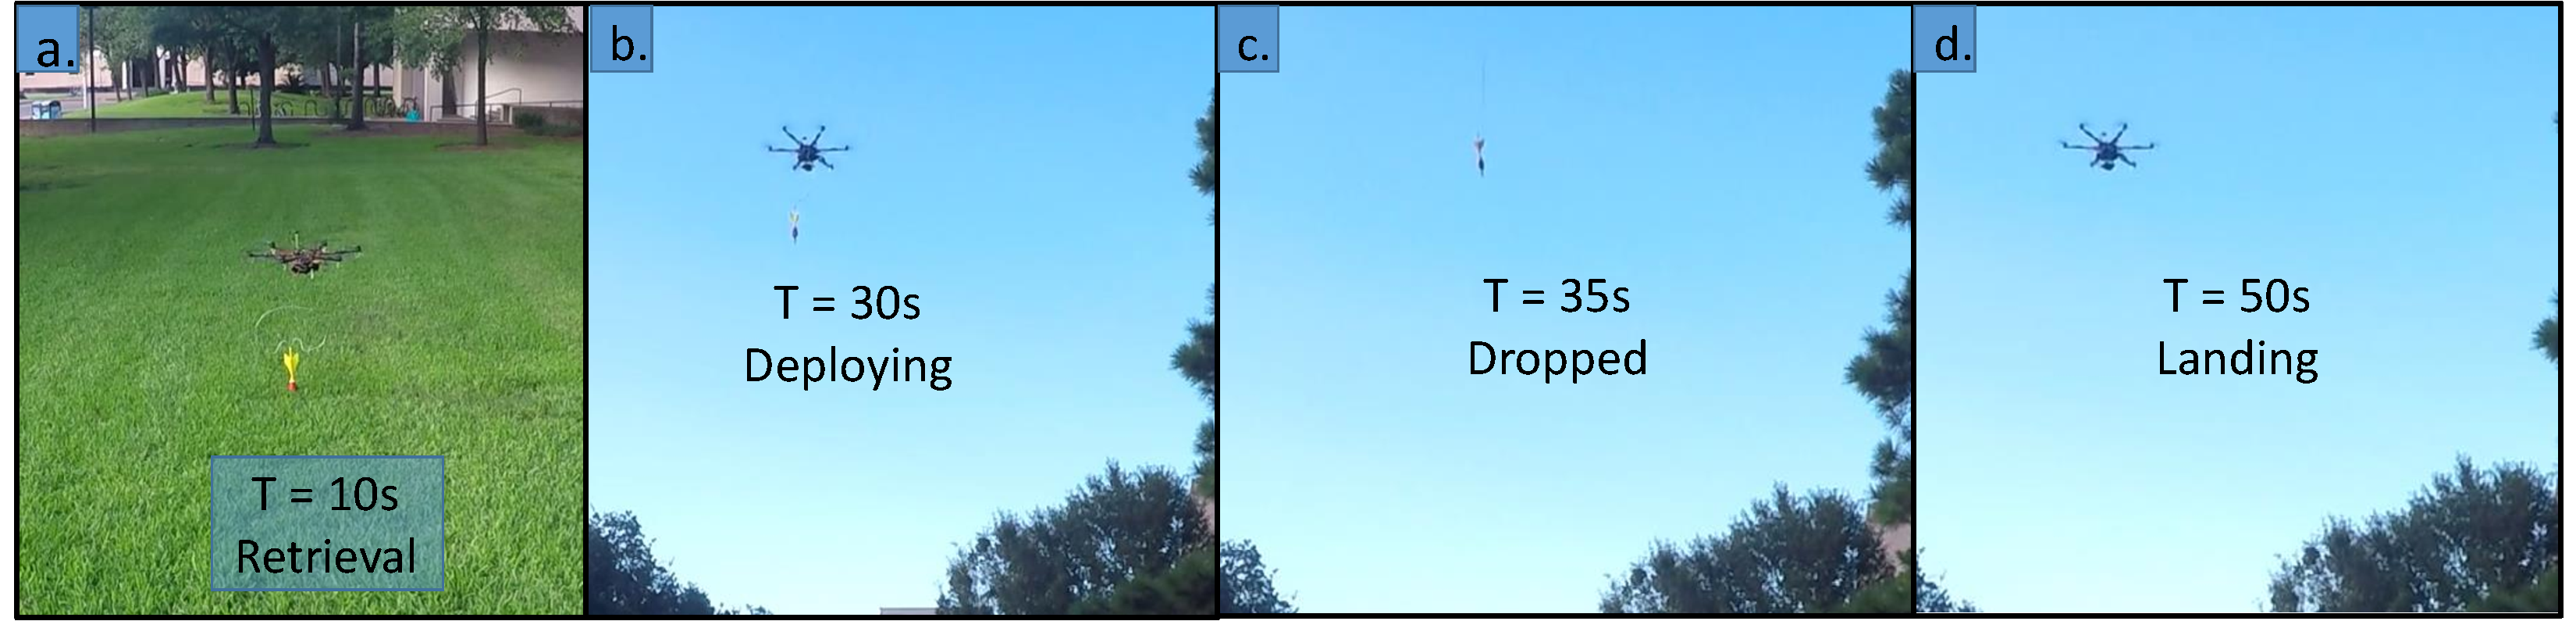
\includegraphics[width=\columnwidth]{SeismicDart_DR.pdf}}
 \caption{SmartDart retrieval and redeployment.  See video attachment. 
 \label{fig:SeismicDart_DR}}
\end{figure}
 